\section{Cuerpo Rígido}

 \capequation{Ecuaciones de cinemática del CR}
     \begin{equation}
     \begin{split}
        \Vec{v}_p &= \Vec{v}_q + \Vec{\Omega} \times \Vec{r}_{p/q}\\
        \Vec{a}_p &= \Vec{a}_q + \Vec{\gamma} \times \Vec{r}_{p/q} + \Vec{\Omega} \times \Vec{v}_{p/q}\\
        \Vec{a}_p &= \Vec{a}_q + \Vec{\gamma} \times \Vec{r}_{p/q} + \Vec{\Omega} \times \vec{\Omega} \times \Vec{r}_{p/q}\\
     \end{split}
     \end{equation}
     \begin{itemize}
         \item Acel. de traslación: \hspace{1cm}$\overrightarrow{a_{p}^{tr}} = \Vec{a}_q$
         \item Acel. tangencial de p: \hspace{0.5cm}$\overrightarrow{a_{p/q}^{tg}} = \Vec{\gamma} \times \Vec{r}_{p/q}$
         \item Acel. centrípeta de p: \hspace{0.5cm}$\overrightarrow{a_{p/q}^{cen}} = \Vec{\Omega} \times \vec{\Omega} \times \Vec{r}_{p/q}$
     \end{itemize}
  
 \capequation{Ecuaciones de Newton del CR}
 \begin{itemize}
     \item Traslación
     \begin{equation}
         \begin{split}
            \sum F_x &= M \cdot a_{cm}^x\\
            \sum F_y &= M \cdot a_{cm}^y\\
            \sum F_z &= M \cdot a_{cm}^z\\
         \end{split}
     \end{equation}
     \item Rotación
     \begin{equation}
         \begin{split}
            \sum \tau_{x}^{cm} &= I_{x}^{cm} \cdot \gamma_{x}\\
            \sum \tau_{y}^{cm} &= I_{y}^{cm} \cdot \gamma_{y}\\
            \sum \tau_{z}^{cm} &= I_{z}^{cm} \cdot \gamma_{z}\\
         \end{split}
     \end{equation}
 \end{itemize}

 \capequation{Gráficos de velocidad/aceleración}
 
    \begin{center}
    \begin{tabular}{>{\centering\arraybackslash}m{1.5in} >{\centering\arraybackslash}m{1.5in}}
    %Traslacion pura
     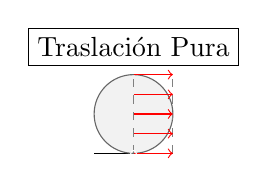
\begin{tikzpicture}
        \node[draw] at (0,1.35) {Traslación Pura};
        \draw (-0.5,0)--(0.5,0);Desliza
        \filldraw[color=black!60, fill=black!5](0,0.5) circle (0.5);
        \draw [gray,dashed] (0.5,0)--(0.5,1);
        \draw [gray,dashed] (0,0)--(0,1);
        \draw [->,red] (0,1)--(0.5,1);
        \draw [->,red] (0,0.75)--(0.5,0.75);
        \draw [->,red] (0,0.5)--(0.5,0.5);
        \draw [->,red] (0,0.25)--(0.5,0.25);
        \draw [->,red] (0,0)--(0.5,0);
        \filldraw[fill opacity=0, black!0 ] (0,0) circle (1pt);
     \end{tikzpicture}
    &
    %Rotacion pura
     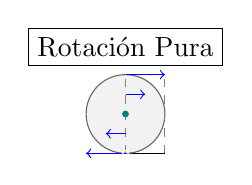
\begin{tikzpicture}
        \node[draw] at (0,1.35) {Rotación Pura};
        \draw (-0.5,0)--(0.5,0);
        \filldraw[color=black!60, fill=black!5](0,0.5) circle (0.5);
        \draw [gray,dashed] (0.5,0)--(0.5,1);
        \draw [gray,dashed] (0,0)--(0,1);
        \draw [->,blue] (0,1)--(0.5,1);
        \draw [->,blue] (0,0.75)--(0.25,0.75);
        \filldraw[teal] (0,0.5) circle (1pt);
        \draw [->,blue] (0,0.25)--(-0.25,0.25);
        \draw [->,blue] (0,0)--(-0.5,0);
        \filldraw[fill opacity=0, black!0 ] (0,0) circle (1pt);
     \end{tikzpicture}
    \\
    %Rototraslacion perfecta
     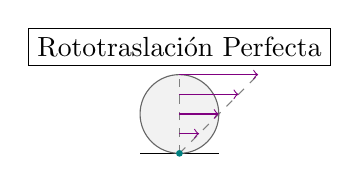
\begin{tikzpicture}
        \draw (-0.5,0)--(0.5,0);
        \filldraw[color=black!60, fill=black!5](0,0.5) circle (0.5);
        \draw [gray,dashed] (0,0)--(1,1);
        \draw [gray,dashed] (0,0)--(0,1);
        \draw [->,violet] (0,1)--(1,1);
        \draw [->,violet] (0,0.75)--(0.75,0.75);
        \draw [->,violet] (0,0.5)--(0.5,0.5);
        \draw [->,violet] (0,0.25)--(0.25,0.25);
        \filldraw[teal] (0,0) circle (1pt);
        \node[draw] at (0,1.35) {Rototraslación Perfecta};
     \end{tikzpicture}
    &
    \vspace{0.5cm}
    %Rototraslacion imperfecta
     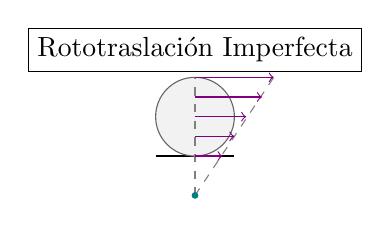
\begin{tikzpicture}
        \node[draw] at (0,1.35) {Rototraslación Imperfecta};
        \draw (-0.5,0)--(0.5,0);
        \filldraw[color=black!60, fill=black!5](0,0.5) circle (0.5);
        \draw [gray,dashed] (0,-0.5)--(1,1);
        \draw [gray,dashed] (0,-0.5)--(0,1);
        \draw [->,violet] (0,1)--(1,1);
        \draw [->,violet] (0,0.75)--(0.85,0.75);
        \draw [->,violet] (0,0.5)--(0.65,0.5);
        \draw [->,violet] (0,0.25)--(0.5,0.25);
        \draw [->,violet] (0,0)--(0.35,0);
        \filldraw[teal] (0,-0.5) circle (1pt);
     \end{tikzpicture}
    \end{tabular}
    \end{center}
    
 \capequation{Centro Instantáneo de Rotación}
    \begin{itemize}
        \item Por definición $v_{cir} := 0_{m/s}$
        \item El CIR coincide con el punto de contacto del cuerpo con la superficie si este se encuentra en un estado de rotación perfecta o bajo condición de rotación sin desplazamiento relativo entre él y la superficie (\textit{RSD})
        \item Útil para ciertos planteos de torques cuando la fuerza que lo realiza es desconocida.
    \end{itemize}
\newpage

 \capequation{Momento de inercia}
 \begin{equation}
        I^{A} = \sum_{i=1}^{\infty} m_i \cdot d^2
 \end{equation}
 \begin{itemize}
    \item Generalización...
    \begin{equation*}
        I^{A} = \int_V \delta \cdot \xi^2 \,dV
    \end{equation*}
    \item En función de $L$...
    \begin{equation}
        I^{A} =\frac{L^A}{\Omega}
    \end{equation}
 \end{itemize}

\capequation{Momentos de inercia notables}
\begin{center}
\begin{tabular}{>{\centering\arraybackslash}m{1.25in} >{\centering\arraybackslash}m{1.25in}}
    Cilindro macizo $I^{cm} = \frac{1}{2} \cdot M \cdot   R ^ 2       $&
    Cilindro hueco  $I^{cm} = \frac{1}{2} \cdot M \cdot  (R ^ 2 + r^2)$
    \\\\
    Esfera maciza $I^{cm} = \frac{2}{5} \cdot M \cdot R ^ 2$&
    Esfera hueca  $I^{cm} = \frac{2}{3} \cdot M \cdot  (R^ 2 + r^2)$
    \\\\
    Barra delgada $I^{cm} = \frac{1}{12} \cdot M \cdot L ^ 2$&
    Aro delgado  $I^{cm} = M \cdot  (R^ 2 + r^2)$
    \\\\
    Partícula $I^{cm} = m \cdot d ^ 2$&
\end{tabular}
\end{center}
 
 \capequation{Teorema de Steiner}
 \begin{equation}
     I^A = I^{cm} + M\cdot d^2
 \end{equation}
 
\capequation{Energía potencial de un CR}
\begin{itemize}
    \item Por ser un CR su Ep es únicamente gravitatoria, si hubiera elástica sería un \textit{soft-body}, es decir, presenta deformaciones.
    \item El CR por ser un tipo de SP, la energía potencial gravitatoria será igual a la mencionada anteriormente
    \begin{equation}
        Ep = M \cdot g \cdot h_{cm}
    \end{equation}    
\end{itemize}

\capequation{Energía cinética de un CR}
\begin{equation}
\begin{split}
    Ec_{_{CR}}^{o} & = \frac{1}{2} \cdot M \cdot v_{cm}^2 + \frac{1}{2} I^{cm} \cdot \Omega^2\\
    Ec_{_{CR}}^o & = Ec_{_{orbital}} + Ec_{_{spin}}\\
    Ec_{_{CR}}^o & = Ec_{_{traslacional}} + Ec_{_{rotacional}}\\
\end{split}
\end{equation}
\begin{itemize}
    \item Si lo analizamos desde el CIR la EC total será la de rotación. Útil para conocer la incógnita de EC total (Recordar aplicar Steiner para 
    conseguir $I^{cir}$)
    \begin{equation}
        Ec_{_{CR}}^{cir} = \frac{1}{2} \cdot I^{cir} \cdot \Omega^2
    \end{equation}
\end{itemize}

\capequation{Energía mecánica de un CR}
\begin{equation}
    Em = M \cdot g \cdot h_{cm} + \frac{1}{2} \cdot M \cdot v_{cm}^2 + \frac{1}{2} I^{cm} \cdot \Omega^2
\end{equation}

\capequation{Trabajo del torque}
\begin{equation}
    W_{\Vec{\tau}_{\vec{F}}^{\ o}} = \int_{\theta_1}^{\theta_2} \Vec{\tau}_{\vec{F}}^{\ o}  \boldsymbol{\cdot} \,d\vec{\theta}
\end{equation}

\capequation{Trabajo de la fuerza de rozamiento}
\begin{itemize}
    \item Si el cuerpo rueda sin deslizar, el trabajo que realiza la fuerza de rozamiento es nulo pues no hay desplazamiento relativo entre la superficie con rozamiento y el cuerpo en cuestión.
    \item Caso contrario, se deberá conocer ``cuanto patina'' para estimar el trabajo de la fuerza de rozamiento.
\end{itemize}

\capequation{Cantidad de movimiento angular del CR}
\begin{equation}
\begin{split}
    \vec{L}^{sist} = \vec{L}^{spin} + \vec{L}^{orbital}\\
    \vec{L}^{sist} = I^{cm} \cdot \Vec{\Omega} + M \cdot \Vec{v}_{cm}
\end{split}
\end{equation}

\begin{equation}
    \vec{L}^{cm} = I^{cm} \cdot \Vec{\Omega}
\end{equation}

\begin{equation}
    \vec{L}^{cir} = I^{cir} \cdot \Vec{\Omega}
\end{equation}


\capequation{Péndulo físico (EDO)}
\begin{equation}
    \frac{d^2 \theta}{dt} + \frac{M\cdot g\cdot d}{I^o} \cdot \sin{\theta} = 0
\end{equation}
\begin{itemize}
    \item Si consideramos ángulos pequeños podemos encontrar la siguiente relación...
    \begin{equation}
        \omega^2 = \frac{M\cdot g\cdot d}{I^o}
    \end{equation}
\end{itemize}

\capequation{Período de un péndulo físico}
\begin{equation}
    T = 2\pi\sqrt{\frac{I^{cm}+M\cdot d^2}{M\cdot g\cdot d}}
\end{equation}

\capequation{Péndulo sincrónico}
\begin{itemize}
    \item Se busca equiparar el período de oscilación de un péndulo físico con uno simple (herramienta útil para medir momentos de inercia).
    \item Se busca la longitud l del péndulo simple que provoque que su período de oscilación sea el mismo que el del CR.
    \item k (Radio de giro baricéntrico) ($k^2 \cdot M = I^{cm}$)
    \item l (Longitud reducida)
    \item d (Distancia del punto propio del CR al centro de rotación)
    \begin{equation}
        l = \frac{k^2}{d} + d
    \end{equation}
\end{itemize}